% -----------------------------------------------------------------------------------------------%

% Oktober 2022
% Template Latex untuk Laporan Kerja Praktek Program Studi Sistem informasi ini
% Dikembangkan oleh Daffa Takratama Savra (daffatakratama13@gmail.com)

% Template ini dikembangkan dari template yang dibuat oleh Inggih Permana (inggihjava@gmail.com).

% Orang yang cerdas adalah orang yang paling banyak mengingat kematian.

% -----------------------------------------------------------------------------------------------%

% -----------------------------------------------------------------------------%
\chapter{\babDua}
% -----------------------------------------------------------------------------%
\section{Profil Instansi}
%-----------------------------------------------------------------------------%
\subsection{Sejarah}
%-----------------------------------------------------------------------------%
Perumahan Kamela Permai merupakan perumahan yang berlokasi di Kecamatan Kuantan Tengah , Kabupaten Kuantan Singingi, Provinsi Riau. Yang dipimpin  oleh Bapak Agusman, S.E selaku Kepala cabang. Cabang Perumahan Kamela Permai ini baru berdiri pada tahun 2023 dengan beberapa pengurus dan staff sebagai berikut:

\begin{figure}
    \centering
    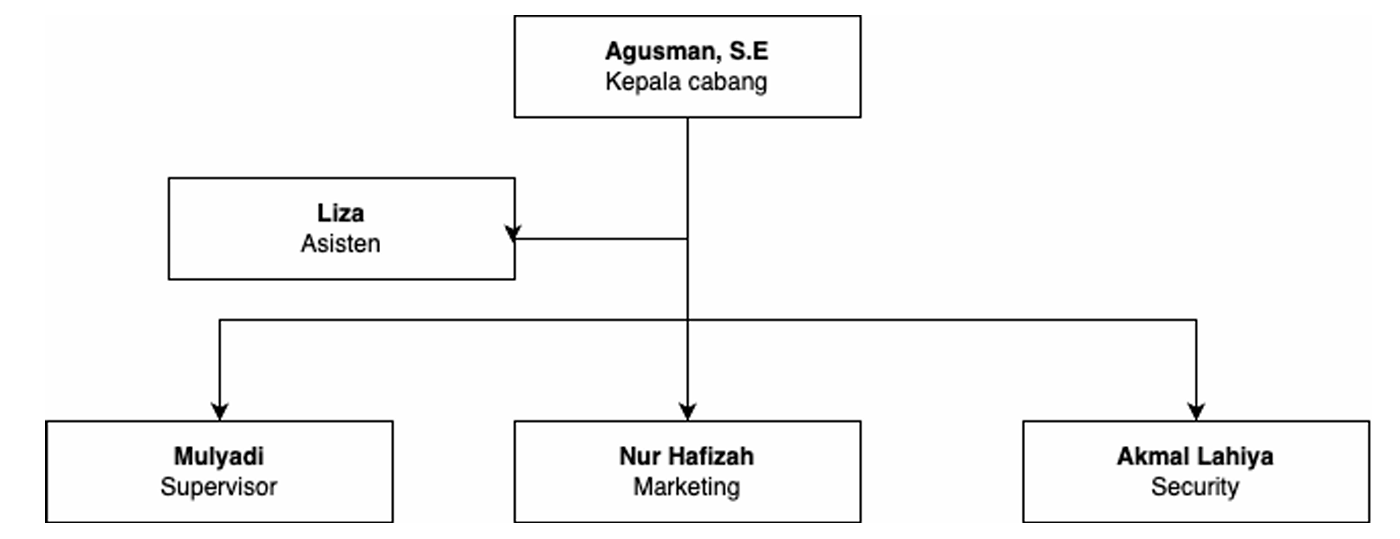
\includegraphics[width=0.75\linewidth]{Struktur Organisasi.png}
    \caption{Struktur Organisasi}
\end{figure}
% -----------------------------------------------------------------------------%
\section{Sistem}
% -----------------------------------------------------------------------------%
Menurut Azhar Susanto dalam bukunya yang berjudul Sistem Informasi Akuntansi: Sistem adalah kumpulan/group dari sub sistem/bagian/komponen apapun baik phisik ataupun non phisik yang saling berhubungan satu sama lain dan bekerja sama secara harmonis untuk mencapai satu tujuan tertentu. Sementara Mohamad Subhan dalam bukunya yang berjudul Analisa Perancangan Sistem mendefinisikan pengertian dari sistem sebagai berikut: Suatu sistem dapat diartikan sebagai suatu kumpulan atau himpunan dari unsur, komponen, atau variabel-variabel yang terorganisasi, saling berinteraksi, saling tergantung satu sama lain dan terpadu. Sistem juga merupakan kumpulan elemen-elemen saling terkait dan bekerja sama untuk memproses masukan (input) yang ditujukan kepada sistem tersebut dan mengolah masukan tersebut sampai menghasilkan keluaran (output) yang diinginkan. Berdasarkan beberapa pendapat yang dikemukakan di atas dapat ditarik kesimpulan bahwa sistem adalah kumpulan bagian-bagian atau sub-sub sistem yang disatukan dan dirancang untuk mencapai suatu tujuan. (Wibawa, 2017).

% -----------------------------------------------------------------------------%
\section{Informasi}
Informasi adalah hasil pemrosesan data yang diperoleh dari setiap elemen sistem tersebut menjadi bentuk yang mudah dipahami dan merupakan pengetahuan yang relevan yang dibutuhkan oleh setiap orang untuk menambah pemahamannya terhadap fakta-fakta yang ada. Informasi bagi setiap elemen akan berbeda satu sama lain sesuai dengan kebutuhannya masing-masing. Ada beberapa definisi informasi menurut para ahli, yakni Menurut (Jogiyanto, 2005), informasi dapat didefinisikan   sebagai data yang diolah menjadi bentuk  yang lebih  berguna  dan  lebih  berarti  bagi yang menerimanya. (Zaliluddin, 2020)
% -----------------------------------------------------------------------------%
\section{Sistem Informasi}
% -----------------------------------------------------------------------------%
Menurut McLeod (2009) Sistem Informasi merupakan sistem yang mempunyai kemampuan untuk mengumpulkan informasi dari semua sumber dan menggunakan berbagai media untuk menampilkan informasi. Menurut Sidharta (1995: 11), “Sebuah sistem informasi adalah sistem buatan manusia yang berisi himpunan terintegrasi dari komponen - komponen manual dan komponen - komponen terkomputerisasi yang bertujuan untuk mengumpulkan data, memproses data, dan menghasilkan informasi untuk pemakai”. Berdasarkan dari beberapa pendapat dapat disimpulkan sistem informasi dapat diartikan sebagai sebuah sistem yang terintegrasi secara optimal dan berbasis komputer yang dapat menghimpun dan menyajikan berbagai jenis data yang akurat untuk berbagai macam kebutuhan. (Firliana et al., 2018).
%-----------------------------------------------------------------------------%

\subsection{Siklus Sistem Informasi}
Siklus Sistem Informasi adalah data yang diolah melalui model menjadi informasi, penerima kemudian menerima informasi tersebut. Membuat suatu keputusan dan melakukan tindakan, yang berarti menghasilkan suatu tindakan yang lain yang akan membuat sejumlah data kembali. Data tersebut akan ditangkap sebagai input, diproses kembali lewat suatu model dan seterusnya membentuk suatu siklus. Siklus ini oleh John Burch disebut dengan siklus informasi \textit{(information cycle)} atau ada yang menyebutkan dengan istilah siklus pengolahan data \textit{(Data processing cycles)}.

\subsection{Komponen Sistem Informasi}
\par Adapun komponen sistem informasi yaitu sebagai berikut:

	\begin{enumerate}
	  	\item Komponen Input/Masukan.
			\par Input merupakan data yang masuk kedalam sistem informasi. Komponen ini merupakan bahan dasar dalam pengolahan informasi. Data untuk sistem informasi perlu ditangkap dan dicatat dalam dokumen dasar. Dokumen dasar merupakan formulir yang digunakan untuk menangkap (capture) dari data yang terjadi, yang selanjutnya data tersebut dimasukkan kedalam sistem informasi \textit{(data entry)}.
	 	 \item Komponen Model.
			\par Informasi yang dihasilkan oleh sistem informasi berasal dari data yang diambil dari basis data yang diolah melalui model-model tertentu.
		\item Komponen Output/Keluaran.
			\par Output adalah produk yang dihasilkan dari sitem informasi yang berguna bagi para pemakainya.
	 	 \item Komponen Teknologi.
			\par Komponen teknologi merupakan komponen penting dalam sistem informasi. Tanpa ada teknologi yang mendukung, maka sistem informasi tidak akan dapat menghasilkan informasi yang tepat waktu.
		\item Komponen Basis Data.
			\par Basis data \textit{(database)} adalah kumpulan dari data yang saling berhubungan satu dengan yang lainnya, tersimpan diperangkat keras komputer dan digunakan perangkat lunak untuk memanipulasinya.
	\end{enumerate}
%-----------------------------------------------------------------------------%
\section{Oktaax}
\par Oktaax merupakan pustaka PHP yang ringan dan dirancang untuk aplikasi berbasis event-driven, yang cocok digunakan untuk aplikasi dengan kebutuhan concurrency tinggi. Pustaka ini memungkinkan pengelolaan koneksi WebSocket secara efisien, mendukung pengembangan aplikasi dengan waktu respons yang cepat, serta mempermudah integrasi dalam server berbasis PHP. Keunggulan utama pustaka ini terletak pada kesederhanaannya dalam penggunaan, memungkinkan pengembangan yang lebih cepat tanpa mengorbankan performa, yang menjadikannya pilihan ideal untuk aplikasi real-time seperti dashboard interaktif \citep{rosyida2021swoole}.
%-----------------------------------------------------------------------------%
\section{Perumahan}
Berdasarkan Undang-undang Nomor 1 tahun 2011 tentang perumahan dan pemukiman. Perumahan adalah kelompok rumah yang berfungsi sebagai lingkungan tempat tinggal atau lingkungan hunian yang dilengkapi dengan sarana dan prasarana lingkungan.
\par Menurut Majalah Properti Indonesia (edisi tahun 2015-2019), konsep perumahan terdiri dari: 
\begin{enumerate}
\item \textit{Eco Living}, Konsep ini memiliki desain yang diatur sedemikian rupa, sehingga sirkulasi udara dan cahaya bisa leluasa.
\item \textit{Custom Homes}, konsep ini menawarkan hunian dengan desain yang dipilih oleh konsumen sesuai dengan selera dan budget.
\item \textit{Tropical Modern Landscape}, konsep ini dirancang dengan unit-unit hunian di dalam perumahan tidak saling menempel antara satu rumah dengan rumah lainnya, sehingga dapat menghadirkan ruang terbuka hijau di samping rumah sekaligus memberikan pencahayaan alami yang maksimal dan memberikan efek visual yang berbeda, 
\item \textit{Urban Smart and Livable}, konsep urban mengadopsi desain arsitektur minimalis.
\end{enumerate}
%-----------------------------------------------------------------------------%
\section{Model Perancangan \textit{Object Oriented Analysis Design} (\textit{OOAD}) }
Metode berorientasi objek atau object oriented merupakan paradigma baru dalam rekayasa perangkat lunak yang memandang sistem sebagai kumpulan objek - objek diskrit yang saling berinteraksi. Yang dimaksud dengan berorientasi objek adalah bahwa mengorganisasikan perangkat lunak sebagai kumpulan objek - objek diskrit yang bekerja sama antara informasi atau struktur data dan perilakau \textit{(behavior)} yang mengaturnya \citep{ariska2016rancang}.
%-----------------------------------------------------------------------------%
\section{\textit{Unified Modelling Language} (\textit{UML})}
Menurut (Sugiarti, 2018) adalah sebuah visualisasi, merancang dan mendokumentasikan sistem piranti lunak. Salah satu standar yang digunakan diperindustrian untuk mengetahui dan mendefinisakan requirement, analisis dan desain, dari suatu arsitektur dalam pemrograman berorientasi objek. (Wahyuni, 2022).
%-----------------------------------------------------------------------------%
\subsection{Diagram \textit{UML} Yang Digunakan}
%-----------------------------------------------------------------------------%
Berikut adalah diagram \textit{UML} yang akan digunakan dalam laporan kerja praktek.
\begin{enumerate}
    \item \textbf{\textit{Use Case Diagram}}\\ \textit{Use Case diagram} merupakan uraian sekelompok yang saling terkait dan membentuk sistem secara teratur yang dilakukan atau diawasi oleh sebuah aktor. \textit{Use Case} atau diagram use case merupakan pemodelan untuk melakukan \textit{(behavior)} sistem informasi yang akan dibuat. (Nuddin \& Fithri, 2015). Tujuan utama permodelan \textit{use case} adalah:

\begin{enumerate} [label=\alph*.]
\item Memutuskan dan mendiskripsikan kebutuhan-kebutuhan fungsional sistem.
\item Memberikan deskripsi jelas dan konsisten dari apa yang seharusnya dilakukan, sehingga model \textit{use case} digunakan diseluruh proses pengembangan untuk komunikasi dan menyediakan basis untuk pemodelan berikutnya yang mengacu sistem harus memberikan fungsionalitas yang dimodelkan para \textit{use case}.
\item Menyediakan basis untuk melakukan pengujian sistem yang memverifikasi sistem. Menguji apakah sistem telah memberikan fungsionalitas yang diminta.
\item Menyediakan kemampuan melacak kebutuhan fungsionalitas menjadi kelas-kelas dan operasi-operasi aktual di sistem. Untuk menyederhanakan perubahan dan ekstensi ke sistem dengan mengubah model use case dan kemudian melacak \textit{use case} yang dipengaruhi ke perancangan dan implementasi sistem.
\end{enumerate}

\par Syarat penamaan \textit{use case} adalah nama didefenisikan sesederhana mungkin dan dapat dipahami, ada dua hal utama pada \textit{use case} yaitu pendefenisian apa yang disebut aktor dan \textit{use case}.

\begin{enumerate} [label=\alph*.]
\item Aktor merupakan orang, proses, atau sistem lain yang berinteraksi dengan sistem informasi yang akan di buat diluar sistem informasi yang akan dibuat sendiri, jadi walaupun simbol dari aktor adalah gambar orang tapi aktor belum tentu orang.
\item  \textit{use case} merupakan fungsionalitas yang disediakan sistem sebagai unit-unit yang saling bertukar pesan antar unit atau aktor.
\end{enumerate}

\captionsetup{position=above} % Mengatur posisi caption di atas
\begin{small}
			\begin{longtable}[c]{|c|>{\centering\arraybackslash}m{2cm}|c|p{7.6cm}|}
			\caption{\textit{Simbol Use Case Diagram}} \label{tab:my-table}\\ % Caption di atas tabel
			\hline
			No & Gambar & Nama & Keterangan \\ \hline
			\endfirsthead
			%
			\endhead
			%
			1 & \parbox[c][2cm][c]{2cm}{\centering 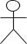
\includegraphics[height=1cm]{useCase/actor.jpg}} & \textit{Actor} & \textit{Use Case} menggambarkan fungsionalitas yang disediakan sistem sebagai unit-unit yang bertukar pesan antar unit dengan aktor, yang dinyatakan dengan menggunakan kata kerja \\ \hline
			
			2 & \raisebox{-.5\height}{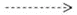
\includegraphics[width=1.5cm]{useCase/dependency.png}} & \textit{Dependency} & Hubungan dimana perubahan yang terjadi pada suatu elemen mandiri (\textit{independent}) akan mempengaruhi elemen yang bergantung padanya, elemen yang tidak mandiri (\textit{independent}). \\ \hline
			3 & \raisebox{-.5\height}{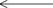
\includegraphics[width=1.5cm]{useCase/generalization.jpg}} & \textit{Generalization} & Hubungan dimana objek anak (\textit{descendent}) berbagi perilaku dan struktur data dari objek yang ada di atasnya objek induk (\textit{ancestor}). \\ \hline
			4 & \raisebox{-.5\height}{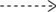
\includegraphics[width=1.5cm]{useCase/include.jpg}} & \textit{Include} & Menspesifikasikan bahwa \textit{use case} sumber secara eksplisit. \\ \hline
			5 & \raisebox{-.5\height}{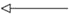
\includegraphics[width=1.5cm]{useCase/extend.png}} & \textit{Extend} & Menspesifikasikan bahwa \textit{use case} target memperluas perilaku dari use case sumber pada suatu titik yang diberikan. \\ \hline
			6 & \raisebox{-.5\height}{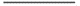
\includegraphics[width=1.5cm]{useCase/association.png}} & \textit{Association} & Apa yang menghubungkan antara objek satu dengan objek lainnya. \\ \hline
			7 & \raisebox{-.5\height}{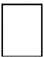
\includegraphics[width=1cm, height=1cm]{useCase/system.png}} & \textit{System} & Menspesifikasikan paket yang menampilkan sistem secara terbatas. \\ \hline
			8 & \raisebox{-.5\height}{
\includegraphics[width=1.5cm]{useCase/use case.jpg}} & \textit{Use Case} & Deskripsi dari urutan aksi-aksi yang ditampilkan sistem yang menghasilkan. \\ \hline
			\end{longtable}
			\end{small}

        \item  \textbf{\textit{Activity Diagram}}\\ \textit{Activity diagram} menggambarkan aliran fungsionalitas dalam suatu sistem informasi. Secara lengkap, \textit{activity diagram} mendefinisikan dimana \textit{workflow} dimulai, dimana berhentinya, aktifitas apa yang terjadi selama \textit{workflow}, dan bagaimana urutan kejadian aktifitas tersebut \citep{dicoding2021activity}. \textit{Activity diagram} juga menyediakan pendekatan untuk proses pemodelan paralel. Bagi mereka yang akrab dengan analisis dan desain struktur tradisional, diagram ini menggabungkan ide-ide yang mendasari diagram alir data dan diagram alur sistem. (Dewi et al., 2012). 

		\par Diagram aktivitas berguna untuk sebagai berikut:
			
			\begin{enumerate} [label=\alph*.]
			\item Rancangan proses bisnis dimana setiap urutan aktivitas yang digambarkan merupakan proses bisnis sistem yang didefenisikan.
			\item Urutan atau pengelompokan tampilan dari sistem atau \textit{user interface} dimana setiap aktivitas di anggap memiliki sebuah rancangan antar muka tampilan.
			\item Rancangan tampilan dimana setiap aktivitas dianggap memerlukan sebuah pengujian yang perlu di defenisikan kasus ujinya.
			\end{enumerate}
        
\begin{small}     
		\begin{longtable}[c]{|c|>{\centering\arraybackslash}m{2cm}|c|p{8cm}|}
		    \captionsetup{position=above} % Menempatkan caption di atas tabel
		    \caption{Simbol \textit{Activity Diagram}} \label{tab:activity-diagram} \\ \hline
		    \textbf{No} & \textbf{Gambar} & \textbf{Nama} & \textbf{Keterangan} \\ \hline
		    \endfirsthead
		    % Tidak ada header lagi di halaman berikutnya
		    \endhead
		    \hline
		    \endfoot
		    % Konten tabel
		    1 & \parbox[c][1.5cm][c]{1.5cm}{\centering 
\includegraphics[width=1.5cm]{activityDiagram/activity.jpg}} & \textit{Activity} & Memperlihatkan bagaimana masing-masing kelas antar muka saling berinteraksi satu sama lain \\ \hline
		    2 & \parbox[c][1.5cm][c]{1.5cm}{\centering 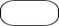
\includegraphics[width=1.5cm]{activityDiagram/action.jpg}} & \textit{Action} & State dari sistem yang mencerminkan eksekusi dari suatu aksi \\ \hline
		    3 & \parbox[c][2cm][c]{2cm}{\centering 
\includegraphics[width=1.5cm]{activityDiagram/initial node.png}} & \textit{Initial Node} & Bagaimana objek dibentuk atau diawali \\ \hline
		    4 & \parbox[c][2cm][c]{2cm}{\centering 
\includegraphics[width=1.5cm]{activityDiagram/activity final node.png}} & \textit{Final Node} & Bagaimana objek dibentuk dan dihancurkan \\ \hline
		    5 & \parbox[c][1.5cm][c]{1.5cm}{\centering 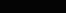
\includegraphics[width=1.5cm]{activityDiagram/fork node.jpg}} & \textit{Fork Node} & Satu aliran yang pada tahap tertentu berubah menjadi beberapa aliran \\ \hline
		\end{longtable}
		\end{small}

    \item \textbf{\textit{Class Diagram}}\\ \textit{Class diagram} adalah salah satu pemodelan yang cukup penting dalam UML, fungsinya adalah untuk membuat sebuat \textit{logical models} dari sebuah sistem \citep{setiawan2021class}. Sebuah class diagram akan menunjukan bagaimana skema dari arsitektur sebuah sistem yang sedang dirancang (Kendal, 2009). \textit{Class diagram} digambarkan dengan class yang berisi atribut dan method, setiap class akan dihubungkan dengan sebuah garis disebut Asosiasi. \citep{aliman2021perancangan}. 
    
\begin{small} % Mengecilkan ukuran font tabel
	\begin{longtable}{|c|>{\centering\arraybackslash}m{2cm}|c|p{7.2cm}|}
	    \captionsetup{position=above} % Menempatkan caption di atas tabel
	    \caption{Simbol \textit{Class Diagram}} \label{tab:Class-Diagram} \\ \hline
	    \textbf{No} & \textbf{Gambar} & \textbf{Nama} & \textbf{Keterangan} \\ \hline
	    \endfirsthead
	    \textbf{No} & \textbf{Gambar} & \textbf{Nama} & \textbf{Keterangan} \\ \hline
	    \endhead
	    \hline
	    \endfoot
	    % Konten tabel
	    1 & \parbox[c][2cm][c]{2cm}{\centering 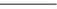
\includegraphics[width=1.5cm, height=1cm]{classDiagram/generalization.jpg}} & \textit{Generalization} & Hubungan dimana objek anak (descendent) berbagi perilaku dan struktur data dari objek yang ada di atasnya, yaitu objek induk (ancestor). \\ \hline
	    2 & \parbox[c][2cm][c]{2cm}{\centering 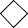
\includegraphics[width=1.5cm]{classDiagram/nary association.png}} & \textit{Nary Association} & Upaya untuk menghindari asosiasi dengan lebih dari dua objek. \\ \hline
	    3 & \parbox[c][2cm][c]{2cm}{\centering 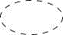
\includegraphics[width=1.5cm]{classDiagram/collaboration.png}} & \textit{Collaboration} & Deskripsi dari urutan aksi-aksi yang ditampilkan sistem, yang menghasilkan suatu hasil yang terukur bagi suatu aktor. \\ \hline
	    4 & \parbox[c][2cm][c]{2cm}{\centering 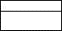
\includegraphics[width=1.5cm]{classDiagram/class.png}} & \textit{Class} & Himpunan dari objek-objek yang berbagi atribut serta operasi yang sama. \\ \hline
	    5 & \parbox[c][2cm][c]{2cm}{\centering 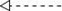
\includegraphics[width=1.5cm]{classDiagram/realization.jpg}} & \textit{Realization} & Operasi yang benar-benar dilakukan oleh suatu objek. \\ \hline
	    6 & \parbox[c][2cm][c]{2cm}{\centering 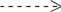
\includegraphics[width=1.5cm]{classDiagram/dependency.jpg}} & \textit{Dependency} & Hubungan dimana perubahan yang terjadi pada suatu elemen mandiri (independent) akan memengaruhi elemen yang bergantung. \\ \hline
	\end{longtable}
	\end{small}

\end{enumerate}
% -----------------------------------------------------------------------------%

\section{Metode \textit{Extreme Programming (XP)}}
% -----------------------------------------------------------------------------%
\par Penelitian ini menggunakan metode pengembangan sistem \textit{Extreme Programming (XP)}. Metode ini cocok untuk pengerjaan perangkat lunak, karena sifat dari metode ini sendiri dilakukan dengan cepat dan juga cenderung menggunakan pendekatan berorientasi objek dan sasaran dari tim yang dibentuk dalam skala kecil melalui tahapan-tahapan yang meliputi Planning (perencanaan), Design (perancangan), Coding (pengkodean), Testing (pengujian) \citep{andriani2023extreme}. 
\textit{Extreme Programming (XP)} merupakan sebuah metode pengembangan perangkat lunak yang mencoba meningkatkan efisiensi dan fleksibilitas dalam suatu pengembangan perangkat lunak yang mengombinasikan berbagai ide sederhana tanpa mengurangi kualitas software yang akan dibangun (Sri Ramadhani dkk., 2019).

\par Adapun tahapan dalam metode \textit{Extreme Programming (XP)} yaitu:

		\begin{enumerate}
			\item \textit{Planning}
			\par Pada tahapan ini merupakan tahapan awal dalam pembangunan sistem dimana dalam tahapan ini dilakukan beberapa kegiatan perencanaan, yaitu, identifikasi permasalahan, menganalisa kebutuhan, sampai dengan penetapan jadwal pelaksanaan pembangunan sistem (Septiani \& Yanti, t.t.).
			\item \textit{Design}
			\par Pada tahapan ini merupakan tahapan perancangan dengan melakukan kegiatan pemodelan yang dimulai dari pemodelan sistem, pemodelan arsitektur sampai dengan pemodelan basis data (Septiani \& Habibie, 2022).
			\item \textit{Coding}
			\par Pada tahapan ini merupakan kegiatan penerapan pemodelan yang sudah dibuat dalam bentuk user interface, dengan menggunakan bahasa pemrograman (Risma dkk., 2021).
			\item \textit{Testing}
			\par Setelah tahapan pengkodean berhasil diselesaikan, kemudian tahapan selanjutnya adalah tahapan pengujian sistem untuk mengetahui kesalahan apa saja yang timbul saat aplikasi sedang berjalan serta mengetahui apakah sistem yang dibangun sudah sesuai dengan kebutuhan pengguna (Marta Syakira, 2022).
		\end{enumerate}
% -----------------------------------------------------------------------------%